\mode*

% Since this a solution template for a generic talk, very little can
% be said about how it should be structured. However, the talk length
% of between 15min and 45min and the theme suggest that you stick to
% the following rules:  

% - Exactly two or three sections (other than the summary).
% - At *most* three subsections per section.
% - Talk about 30s to 2min per frame. So there should be between about
%   15 and 30 frames, all told.


\section{Logging}

\subsection{Securing Logging Mechanisms}

\begin{frame}
  \begin{itemize}
    \item Have a process write log messages to a file.

    \item Then the running process must access the file.
      \begin{itemize}
        \item Could be done using append only access, thus no reading or 
          rewriting.

        \item Could trust the process to do a setuid(2) system call.

        \item This saves us from trusting the user -- but only if the user 
          doesn't have access to the hardware.

      \end{itemize}

    \item We could also log to this or another system via syslog(3), this helps 
      us if we don't trust the user or the process.

    \item However, the problem remains with the sysadmin who has superuser 
      access to the system.

  \end{itemize}
\end{frame}

\begin{frame}
  \begin{itemize}
    \item The sysadmin problem can be solved using a clever setup of separation 
      of duty.

    \item E.g.\ the logs of sysadmin \(A\) will be stored under the control of 
      sysadmins \(B\) and \(C\).

    \item This way sysadmin \(A\) can do everything except modify his own 
      logging mechanisms.

    \item The downside of this is that all systems must be online for this to 
      work.

  \end{itemize}
\end{frame}

\subsection{Schneier-Kelsey Logs}

\begin{frame}
  \begin{itemize}
    \item The Schneier-Kelsey logging scheme provides a secure logging 
      mechanism for storing logs in an untrusted machine.

    \item The untrusted machine \(\U\) is expected to work correctly up to 
      a time \(t\) when it is compromised by an attacker.

    \item The logging mechanism and the integrity of the logs \(L_1, \ldots, 
      L_{t-1}\) before \(t\) are provided with confidentiality and integrity.

    \item All logs \(L_t, L_{t+1}, \ldots\) generated from this point, however, 
      are under the influence of the attacker.

  \end{itemize}
\end{frame}

\begin{frame}
  \begin{itemize}
    \item The scheme consists of an untrusted principal \(\U\) and a trusted 
      principal \(T\).

  \end{itemize}
\end{frame}

\begin{frame}
  \begin{figure}
    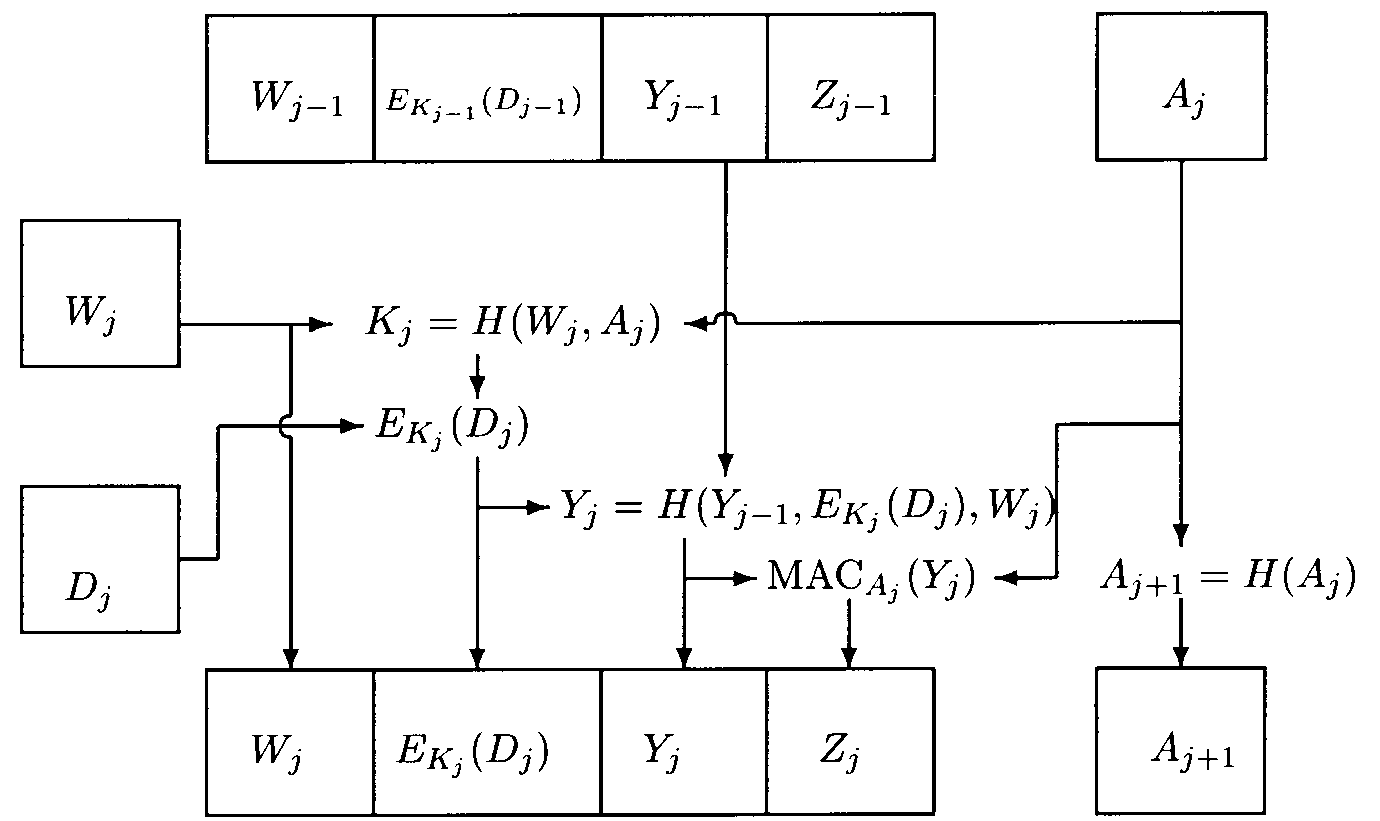
\includegraphics[height=0.7\textheight]{seclog.png}
    \caption{%
      Overview of Schneier-Kelsey secure-log scheme; where \(W_j\) is the type 
      of entry, \(D_j\) is entry data, \(K_j\) is entry key, \(A_j\) is 
      authentication key, and \(H\) is a one-way function.
      Image:~\cite{schneier1999secure}.
    }
  \end{figure}
\end{frame}

\begin{frame}
  \begin{itemize}
    \item One interesting property is that validation of logs can be delegated 
      to a third party verifier \(\V\).
  \end{itemize}
\end{frame}


%%%%%%%%%%%%%%%%%%%%%%

\begin{frame}
  \small
  \printbibliography{}
\end{frame}

